\section{Nonlinear Latent Variable Models}

  Now we will consider ourselves with nonlinear latent variables models, which still defines a simple latent random variable $Z$ with prior $p(z)$, but now a family of nonlinear functions $\{f_\theta (z)\}$ that defines the generative component $f_\theta (x \mid z)$. In factor models, we have taken linear transformations of random variables and therefore the likelihood had been easy to calculate, differentiate, and therefore optimize. 

  In the general nonlinear case, we usually deal with $f_\theta$ not as a transformation of $Z$ to $X$, but really $f_\theta (z)$ becomes the \textit{parameters} of $X \mid Z = z$. This allows to define the \textit{implicitly parameterized} family of distributions $\{p_\theta\}$. Given that the true distribution of the data is $p^\ast (x)$, we would like to find a distribution $p_\theta (x)$ that is a good approximation. 
  \begin{equation}
    p^\ast (x) \approx p_\theta (x)
  \end{equation}
  To calculate the likelihood $p_\theta (x)$, we must compute the marginal 
  \begin{equation}
    p_\theta (x) = \int p_\theta (x, z) \,dz = \int p_\theta (x \mid z) \, p(z) \,dz
  \end{equation}
  which is known to be computationally intractable due to the integral. At first, it seems like all hope is lost, but statisticians have a few tricks up their sleeves. 
  \begin{enumerate} 
    \item The first trick is to notice that by Bayes rule, we can compute the likelihood not as an integral, but as 
    \begin{equation}
      p_\theta (x) = \frac{p_\theta (x \mid z) \, p(z)}{p_\theta (z \mid x)} 
    \end{equation}
    So it suffices to find a good approximation of $p_\theta (z \mid x)$, which is a probabilistic discriminative model for the latent variable (i.e. we are trying to compute the distribution of $z$ given $x$ as if we were predicting it). We can do MCMC since $p_\theta (z \mid x) \propto p_\theta (x \mid z) \, p(z)$, but often this can be slow to fit. 

    \item The next trick is called the variational lower bound, which is a lower bound on the log likelihood, and therefore by optimizing it we can hope to optimize the log-likelihood as well. This works well in practice. 

    \item The next trick is by optimizing the Fisher score, which is the gradient of the log likelihood \textit{with respect to the covariates} (not the parameters!). 
  \end{enumerate}

\subsection{Variational Lower Bounds} 

  We focus on this problem and define a family of distributions $\{q_\phi (z \mid x)\}_\phi$ and use it to approximate $p_\theta (z \mid x)$. Therefore, searching for a good $\phi$ and therefore a good $q_\phi$ is basically the problem of \textbf{variational Bayesian inference}. Essentially we are trying to construct an encoder and a decoder.

  \begin{figure}[H]
    \centering 
    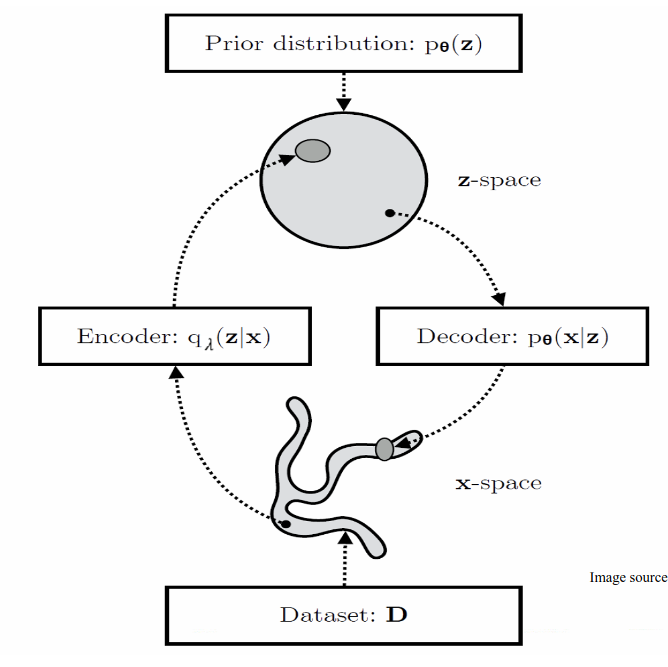
\includegraphics[scale=0.4]{img/latent_variable_model.png}
    \caption{If $q_{\phi} = p_{\theta}$, then the diagram commutes, i.e. $p(z) p_{\theta}(x \mid z) = p(x) p_{\theta}(z \mid x) = p_{\theta} (x, z)$.} 
    \label{fig:latent_variable_model}
  \end{figure}

  As we have stated before (and in pretty much all density estimation problems), our job is to maximize the log likelihood of the training set: 
  \begin{equation}
    \sum_{i} \log p(x^{(i)})
  \end{equation}

  In order to do this for this problem, we need a little fact from information theory. 

  \begin{theorem}[Log Likelihood vs Conditional Entropy]
    The KL divergence can be decomposed to 
    \begin{equation}
      KL \big( q_\phi (z \mid x) \mid\mid p_{\theta} (z \mid x) \big) = \mathbb{E}_{q_\phi(z \mid x)} [ \log q_{\phi} (z \mid x)] + \log p_{\theta} (x) - \mathbb{E}_{q_{\phi} (z \mid x)} [\log p_{\theta} (x, z)]
    \end{equation}
    and hence 
  \end{theorem}
  \begin{proof}
    Starting with the definition of KL divergence:
    \begin{align}
      KL(q_\phi(z \mid x) \mid\mid p_\theta(z \mid x)) &= \mathbb{E}_{q_\phi(z \mid x)}\left[\log \frac{q_\phi(z \mid x)}{p_\theta(z \mid x)}\right] \\
      &= \mathbb{E}_{q_\phi(z \mid x)}[\log q_\phi(z \mid x)] - \mathbb{E}_{q_\phi(z \mid x)}[\log p_\theta(z \mid x)]
    \end{align}

    By Bayes' rule, we know that
    \begin{equation}
      p_\theta(z \mid x) = \frac{p_\theta(x, z)}{p_\theta(x)}
    \end{equation}

    Substituting this into our equation gives 
    \begin{align}
      KL(q_\phi(z \mid x) \mid\mid p_\theta(z \mid x)) &= \mathbb{E}_{q_\phi(z \mid x)}[\log q_\phi(z \mid x)] - \mathbb{E}_{q_\phi(z \mid x)}\left[\log \frac{p_\theta(x, z)}{p_\theta(x)}\right] \\
      &= \mathbb{E}_{q_\phi(z \mid x)}[\log q_\phi(z \mid x)] - \mathbb{E}_{q_\phi(z \mid x)}[\log p_\theta(x, z)] + \mathbb{E}_{q_\phi(z \mid x)}[\log p_\theta(x)]
    \end{align}

    Since $\log p_\theta(x)$ is constant with respect to $z$, we can take it out of the expectation. 
    \begin{equation}
      \mathbb{E}_{q_\phi(z \mid x)}[\log q_\phi(z \mid x)] - \mathbb{E}_{q_\phi(z \mid x)}[\log p_\theta(x, z)] + \log p_\theta(x)
    \end{equation}
  \end{proof}

  Therefore maximizing the log-likelihood is equivalent to minimizing the KL-divergence. 
  \begin{equation}
    \log p_\theta (x) = KL \big( q_\phi (z \mid x) \mid\mid p_{\theta} (z \mid x) \big) + \mathbb{E}_{q_{\phi} (z \mid x)} [\log p_{\theta} (x, z)] - \mathbb{E}_{q_\phi(z \mid x)} [ \log q_{\phi} (z \mid x)]
  \end{equation}
  But again the KL divergence part is intractable due to $p_\theta (z \mid x)$ being intractable. Using the fact that the KL divergence is always greater than or equal to $0$, we can drop the term and set a lower bound on the log likelihoods. This lower bound is called the \textit{variational lower bound}.  
  \begin{equation}
    \sum_{i=1}^N \log p_{\theta} (x^{(i)}) \geq \sum_{i=1}^N \mathbb{E}_{q_\phi (z \mid x^{(i)})} [ \log p_{\theta} (x^{(i)}, z)] - \sum_{i=1}^N \mathbb{E}_{q_{\phi} (z \mid x^{(i)})} [ \log q_{\phi} (z \mid x^{(i)}) ]
  \end{equation} 

  \begin{definition}[Variational Lower Bound]
    The \textbf{variational lower bound} of the dataset $\mathcal{D}$ is defined 
    \begin{equation}
      \elbo(\mathcal{D}, \phi, \theta) = \sum_{i=1}^N \mathbb{E}_{q_\phi (z \mid x^{(i)})} [ \log p_{\theta} (x^{(i)}, z)] - \sum_{i=1}^N \mathbb{E}_{q_{\phi} (z \mid x^{(i)})} [ \log q_{\phi} (z \mid x^{(i)})] 
    \end{equation}
    which can be decomposed into the sums of the variational lower bounds of the individual data points. 
    \begin{equation}
      \elbo(\mathcal{D}, \phi, \theta) = \sum_i \elbo(x^{(i)}, \phi, \theta) 
    \end{equation}
    where 
    \begin{equation}
      \elbo(x^{(i)}, \phi, \theta) = \mathbb{E}_{q_\phi (z \mid x^{(i)})} [ \log p_{\theta} (x^{(i)}, z)] - \mathbb{E}_{q_{\phi} (z \mid x^{(i)})} [ \log q_{\phi} (z \mid x^{(i)})] 
    \end{equation}
  \end{definition}

  Note that we can alternatively define ELBO using Jensen's inequality. 

  \begin{definition}[Evidence Lower Bound]
    To lower bound it, we can use Jensen's inequality\footnote{Given convex function $f: \mathbb{R} \rightarrow \mathbb{R}$, and random variable $X$, $\mathbb{E}[f(x)] \geq f(\mathbb{E}[X])$.} with the concave function $f(x) = \log(x)$ over domain $\mathbb{R}^+$ and the following holds true for all $\theta$ and more importantly, for \textit{any arbitrary density function} $q(z)$. Therefore, we have 
    \begin{align}
      \ell(\theta) & = \log p_\theta (x) \\
                   & = \log \int p_\theta (x, z) \,dz \\
                   & = \log \int q_\phi (z) \frac{p_\theta (x, z)}{q_\phi (z)} \,dz \\ 
                   & \geq \int q_\phi (z \mid x) \log \bigg( \frac{p_\theta (x, z)}{q_\phi (z)} \bigg) \,dz \\  
                   & = \elbo(x, q_\phi)
    \end{align}
    The lower bound is called the \textbf{evidence lower bound (ELBO)}, and the ELBO of the whole dataset is 
    \begin{equation}
      \elbo(\mathcal{D}, \phi, \theta) = \sum_{i=1}^N \elbo(x^{(i)}, \phi, \theta)
    \end{equation}
  \end{definition} 

  Note that this lower bound is with respect to \textit{any} distribution $q_\phi$, and it is because of this flexibility that we choose $q_\phi$ in the first place. Therefore, we can vary $\phi$ in hopes that the lower bound is maximized, and optimize with respect to this, hence the name \textit{variational}. For more interpretability, look at the corollary. 

  \begin{corollary}[Decomposition of ELBO]
    The following decomposition of ELBO shows that maximizing the ELBO simultaneously attempts to keep $q_\phi$ close to $p$ and concentrate $q_\phi(z \mid x)$ on those $z$ that maximizes $\ln p_\theta (x \mid z)$. That is, the approximate posterior $q_\phi$ balances between staying close to the prior $p(z)$ and moving towards the maximum likelihood $\argmax_z \ln p_\theta (x \mid z)$. 
    \begin{equation}
      \elbo(x^{(i)}, \phi, \theta) = \underbrace{\mathbb{E}_{q_\phi (z \mid x^{(i)})} [\log p_{\theta} (x^{(i)} \mid z)]}_{\substack{\text{likelihood term} \\ \text{(reconstruction part)}}}- \underbrace{KL(q_{\phi} (z \mid x^{(i)}) \mid\mid p(z))}_{\substack{\text{closeness of encoding to } p(z) \\ \text{(typically Gaussian)}}}
    \end{equation}
    Note the first expression is the likelihood term, which measures the reconstruction quality of the decoder $p_\theta(x^{(i)} \mid z)$ averaged over encodings sampled from $q_\phi(z \mid x^{(i)})$. The second term is the KL divergence between the encoder distribution $q_\phi(z \mid x^{(i)})$ and the prior $p(z)$, which acts as a regularizer by ensuring the encoded distributions remain close to the chosen prior, typically a standard normal distribution.
  \end{corollary}
  \begin{proof}
    Starting with the ELBO for a single data point:
    \begin{align*}
      \elbo(x^{(i)}, \phi, \theta) &= \mathbb{E}_{q_\phi(z \mid x^{(i)})}[\log p_\theta(x^{(i)}, z)] - \mathbb{E}_{q_\phi(z \mid x^{(i)})}[\log q_\phi(z \mid x^{(i)})]
    \end{align*}

    Using the chain rule of probability for the joint distribution:
    \begin{align*}
      p_\theta(x^{(i)}, z) = p_\theta(x^{(i)} \mid z)p(z)
    \end{align*}

    Substituting this into our ELBO:
    \begin{align*}
      \elbo(x^{(i)}, \phi, \theta) &= \mathbb{E}_{q_\phi(z \mid x^{(i)})}[\log p_\theta(x^{(i)} \mid z) + \log p(z)] - \mathbb{E}_{q_\phi(z \mid x^{(i)})}[\log q_\phi(z \mid x^{(i)})] \\
      &= \mathbb{E}_{q_\phi(z \mid x^{(i)})}[\log p_\theta(x^{(i)} \mid z)] + \mathbb{E}_{q_\phi(z \mid x^{(i)})}[\log p(z)] - \mathbb{E}_{q_\phi(z \mid x^{(i)})}[\log q_\phi(z \mid x^{(i)})] \\
      &= \mathbb{E}_{q_\phi(z \mid x^{(i)})}[\log p_\theta(x^{(i)} \mid z)] - \left(\mathbb{E}_{q_\phi(z \mid x^{(i)})}[\log q_\phi(z \mid x^{(i)})] - \mathbb{E}_{q_\phi(z \mid x^{(i)})}[\log p(z)]\right) \\
      &= \underbrace{\mathbb{E}_{q_\phi(z \mid x^{(i)})}[\log p_\theta(x^{(i)} \mid z)]}_{\text{reconstruction term}} - \underbrace{KL(q_\phi(z \mid x^{(i)}) \mid\mid p(z))}_{\text{KL divergence term}}
    \end{align*}
  \end{proof} 

  Therefore, maximizing the ELBO will simultaneously allow us to obtain an accurate generative model $p_\theta (x \mid z) \approx p^\ast (x \mid z)$ and an accurate discriminative model $q_\phi (z \mid x) \approx p_\theta (z \mid x)$. The next step is to actually maximize the ELBO with respect to both $\theta$ and $\phi$. To do this we need to compute the derivatives of $\elbo$ w.r.t. to $\phi$ and $\theta$. 

  \begin{equation}
    \max_{\phi, \theta} \elbo(\mathcal{D}, \phi, \theta)
  \end{equation}
  It turns out that this itself is a nonconvex optimization problem, and to make it doable we iterate between updating $\phi$ and $\theta$. Remember that the ELBO is really an expectation, i.e. an integral, and to get a good estimate of its derivative we must try to change it from the derivative of an expectation to the expectation of a derivative. The gradient with respect to $\theta$ is very easy since from measure theory, we are deriving and integrating over different variables. 

  \begin{lemma}[Gradient of ELBO w.r.t. $\theta$]
    For $\theta$, its unbiased gradient is 
    \begin{equation}
      \nabla_\theta \elbo(x, \theta, \phi) = \mathbb{E}_{q_\phi (z \mid x)} \big[ \nabla_\theta \log p_\theta (x \mid z) \big]
    \end{equation}
    and therefore we can approximate the gradient by sampling $L$ points $p^{(1)}, \ldots, p^{(L)}$ from $p(z)$ and computing the gradient of the log (since we know the closed form of the conditional distribution given $z$), and finally averaging them. 
    \begin{equation}
      \nabla_\theta \elbo(x, \theta, \phi) \approx \frac{1}{L} \sum_{l=1}^L \nabla_\theta \log p_\theta (x \mid z^{(l)})
    \end{equation}
    which is guaranteed to converge by the law of large numbers, and furthermore, we can do this for any batch size $L$.  
  \end{lemma}
  \begin{proof}
    Note that the KL divergence does not depend on $\theta$ and neither does the prior, so they can be removed 
    \begin{align} 
      \nabla_\theta \elbo(x, \theta, \phi) & = \nabla_\theta \big\{ \mathbb{E}_{q_\phi (z \mid x)} [ \log p_\theta (x, z)] - \mathbb{E}_{q_\phi (z \mid x)} [\log q_{\phi} (z \mid x)] \} \\ 
                                           & = \nabla_\theta \big\{ \mathbb{E}_{q_\phi (z \mid x)} [ \log p_\theta (x, z)] \} \\ 
                                           & = \mathbb{E}_{q_\phi (z \mid x)} \big[ \nabla_\theta \{ \log p_\theta (x, z) \big] \\
                                           & = \mathbb{E}_{q_\phi (z \mid x)} \big[ \nabla_\theta \{ \log p_\theta (x \mid z) - \log p_(z) \} \big] \\
                                           & = \mathbb{E}_{q_\phi (z \mid x)} \big[ \nabla_\theta \log p_\theta (x \mid z) \big] 
    \end{align}
  \end{proof}

  However, taking the gradient w.r.t. $\phi$ is more complicated since we cannot put the gradient in the expectation, i.e. swap the derivative and integral (since we are deriving and integrating w.r.t. $\phi$). Fortunately, we have a well-known mathematical identity often used in policy gradient algorithms in reinforcement learning. \cite{W92} 

  \begin{lemma}[Log-Derivative Trick]
    The following identity holds. 
    \begin{equation}
      \nabla_\phi \mathbb{E}_{q_\phi(z)}[f(z)] = \mathbb{E}_{q_\phi(z)}[f(z)\nabla_\phi \log q_\phi(z)]
    \end{equation}
  \end{lemma}
  \begin{proof}
    First, let's write out the left-hand side using the definition of expectation:
    \begin{align*}
    \nabla_\phi \mathbb{E}_{q_\phi(z)}[f(z)] &= \nabla_\phi \int f(z)q_\phi(z)dz
    \end{align*}

    Under suitable regularity conditions, we can exchange the gradient and integral operators:
    \begin{align*}
    &= \int f(z)\nabla_\phi q_\phi(z)dz
    \end{align*}

    Now, we multiply and divide by $q_\phi(z)$ inside the integral:
    \begin{align*}
    &= \int f(z) q_\phi(z) \frac{\nabla_\phi q_\phi(z)}{q_\phi(z)} dz
    \end{align*}

    Recognize that $\nabla_\phi \log q_\phi(z) = \frac{\nabla_\phi q_\phi(z)}{q_\phi(z)}$ by the chain rule:
    \begin{align*}
    &= \int f(z) q_\phi(z) \nabla_\phi \log q_\phi(z) dz
    \end{align*}

    Finally, we can rewrite this back as an expectation:
    \begin{align*}
    &= \mathbb{E}_{q_\phi(z)}[f(z)\nabla_\phi \log q_\phi(z)]
    \end{align*}
  \end{proof}

  \begin{example}[Gradient of Expection of $f(x) = x^2$ w.r.t. Gaussian]
    Assume we have a normal distribution $q$ that is parameterized by $\phi$, specifically
    $q_\phi(x) = N(\phi, 1)$. We want to solve the below problem
    \begin{equation}
      \min_\phi \mathbb{E}_q[x^2]
    \end{equation}

    This is of course a rather silly problem and the optimal $\phi = 0$ is obvious. One way to calculate $\nabla_\phi \mathbb{E}[x^2]$ is using the log-derivative trick as follows
    \begin{align}
      \nabla_\phi \mathbb{E}_q[x^2] &= \nabla_\phi\int q_\phi(x)x^2dx \\
      &= \int x^2\nabla_\phi q_\phi(x)\frac{q_\phi(x)}{q_\phi(x)}dx \\
      &= \int q_\phi(x)\nabla_\phi\log q_\phi(x)x^2dx \\
      &= \mathbb{E}_q[x^2\nabla_\phi\log q_\phi(x)]
    \end{align}

    For our example where $q_\phi(x) = N(\phi, 1)$, this method gives
    \begin{equation}
      \nabla_\phi \mathbb{E}[x^2] = \mathbb{E}_q[x^2(x-\phi)]
    \end{equation}
  \end{example}

  Using this on the gradient of ELBO w.r.t. $\phi$ gives the following form as the expectation of the gradient. 

  \begin{lemma}
    We can use the score function estimator. 
    \begin{align}
      \nabla_\phi \elbo(x, \theta, \phi) & = \nabla_\phi \mathbb{E}_{q_\phi(z|x)}[\log p_\theta(x,z) - \log q_\phi(z|x)] \\
                                         & = \mathbb{E}_{q_\phi(z|x)}\big[ \nabla_\phi \big\{ \log q_\phi(z|x)(\log p_\theta(x,z) - \log q_\phi(z|x)) \big\} \big]
    \end{align}
  \end{lemma}
  \begin{proof}
  \end{proof}

  However, REINFORCE is known to have high variance, and so we need large batch sizes $L$ for good convergence. Many methods such as $\cite{reduce, reduce2}$ were developed to reduce this. Later it was shown in \cite{vae1} that the \textit{reparamaterization trick} beat everything else, allowing us to efficiently train neural-net-based nonlinear latent variable models, e.g. the variational autoencoder. We will focus on the reparameterization trick in my deep learning notes and omit it here.  Now that we have approximate closed form solutions for the gradients, we can optimize the two using coordinate ascent. Note that we have shown this for a single sample $x$, and ideally we would do this for a minibatch of samples $x^{(i)}$. 

  \begin{algo}[Coordinate Ascent Variational Inference]
    A common approach to maximize the ELBO is coordinate ascent, where we alternatively optimize with respect to $\phi$ and $\theta$:

    \begin{algorithm}[H]
      \caption{Coordinate Ascent Variational Inference (CAVI) with Reparameterization}
      \begin{algorithmic}[1]
        \Require Initial parameters $\theta^{[0]}$, $\phi^{[0]}$, batch size B, number of samples L
        \While{not converged}
          \State // E-step: optimize variational parameters
          \State Sample minibatch $\{x^{(1)}, \ldots, x^{(B)}\}$ from dataset $\mathcal{D}$
          \State Sample noise $\{\epsilon^{(1)}, \ldots, \epsilon^{(L)}\} \sim p(\epsilon)$ for reparameterization
          \State Transform noise to latent variables: $z^{(l)} = g_{\phi^{[t]}}(\epsilon^{(l)}, x)$ for $l=1,\ldots,L$
          \State // Approximate gradient using Monte Carlo samples
          \State $\hat{g}_\phi \gets \frac{1}{BL} \sum_{i=1}^B \sum_{l=1}^L [\nabla_\phi \log p_{\theta^{[t]}}(x^{(i)} \mid z^{(l)}) - \nabla_\phi \log q_{\phi^{[t]}}(z^{(l)} \mid x^{(i)}) + \nabla_\phi \log p(z^{(l)})]$
          \State $\phi^{[t+1]} \gets \phi^{[t]} + \eta_\phi \hat{g}_\phi$ \Comment{Update with learning rate $\eta_\phi$}
          \State // M-step: optimize model parameters
          \State $\hat{g}_\theta \gets \frac{1}{BL} \sum_{i=1}^B \sum_{l=1}^L \nabla_\theta \log p_{\theta^{[t]}}(x^{(i)} \mid z^{(l)})$
          \State $\theta^{[t+1]} \gets \theta^{[t]} + \eta_\theta \hat{g}_\theta$ \Comment{Update with learning rate $\eta_\theta$}
        \EndWhile
      \end{algorithmic}
    \end{algorithm}
  \end{algo} 

  Once we are done, we have our optimized encoder and decoders $p_\theta$ and $q_\phi$. 

\subsection{EM Algorithm} 

  Let's consider a slightly simpler sub-problem where we have covariates $x^{(i)} \sim X$ coming from distribution $p(x)$. We can again add latent random variables $Z$ but rather than being fixed, the prior $p_\theta (z)$ is also parameterized by $\theta$. Therefore, we would like to find 
  \begin{equation}
    \argmax_\theta p_\theta (x) = \argmax_\theta \int p_\theta (x \mid z) \, p_\theta (z) \,dz
  \end{equation} 
  Even though this integral is not tractable, we will assume that $p_\theta (z \mid x)$ can be computed for a given $\theta$. Let's try to redo our algorithm again with computable posterior assumptions. We have a training set $\mathcal{D} = \{x^{(i)}\}_{i=1}^n \in \mathbb{R}^d$, which we assume are generated by some latent distributions $p_\theta (z)$ followed by the generative component $p_\theta (x \mid z)$. Then, we bound the likelihood of each sample $x^{(i)}$ by an ELBO that varies for all distributions $q^{(i)}$ (we write $q$ rather than $q_\phi$ since the $\phi$ will be irrelevant here). 
  \begin{equation}
    \log p_{\theta} (x^{(i)}) \geq \elbo(x^{(i)}, q^{(i)}, \theta) = \mathbb{E}_{q^{(i)} (z \mid x^{(i)})} [ \log p_{\theta} (x^{(i)}, z)] - \mathbb{E}_{q^{(i)} (z \mid x^{(i)})} [ \log q^{(i)} (z \mid x^{(i)}) ]
  \end{equation} 
  Summing this all up gives the ELBO of our dataset, which is a lower bound for \textit{all} collections of distributions $q^{(1)}, \ldots, q^{(n)}$. 
  \begin{align}
    \sum_{i=1}^N \log p_{\theta} (x^{(i)}) & \geq \elbo(\mathcal{D}, q^{(1)}, \ldots, q^{(n)}, \theta) \\ 
                                           & = \sum_{i=1}^N \mathbb{E}_{q^{(i)} (z \mid x^{(i)})} [ \log p_{\theta} (x^{(i)}, z)] - \sum_{i=1}^N \mathbb{E}_{q^{(i)} (z \mid x^{(i)})} [ \log q^{(i)} (z \mid x^{(i)}) ]
  \end{align} 
  We maximized the ELBO w.r.t. $q$ and $\theta$ by using CAVI, but by invoking our assumption that the posterior $p_\theta (z \mid x)$ can be computed, we can immediately find a maximum. 

  \begin{theorem}[Posterior Maximizes ELBO] 
    When we set $q^(i) (z \mid x) = p(z \mid x^{(i)})$, equality is achieved. 
    \begin{align}
      \sum_{i=1}^N \log p_{\theta} (x^{(i)}) & = \elbo(\mathcal{D}, q^{(1)}, \ldots, q^{(n)}, \theta) \\ 
                                             & = \sum_{i=1}^N \mathbb{E}_{q^{(i)} (z \mid x^{(i)})} [ \log p_{\theta} (x^{(i)}, z)] - \sum_{i=1}^N \mathbb{E}_{q^{(i)} (z \mid x^{(i)})} [ \log q^{(i)} (z \mid x^{(i)}) ]
    \end{align}
  \end{theorem}
  \begin{proof}
    Let's start by examining the gap between $\log p_\theta(x^{(i)})$ and the ELBO. From our previous derivations, this gap is the KL divergence:
    \begin{align}
      \log p_\theta(x^{(i)}) - \elbo(x^{(i)}, q^{(i)}, \theta) &= KL(q^{(i)}(z|x^{(i)}) \| p_\theta(z|x^{(i)})) \\
      &= \mathbb{E}_{q^{(i)}}[\log q^{(i)}(z|x^{(i)}) - \log p_\theta(z|x^{(i)})]
    \end{align}

    When we set $q^{(i)}(z|x^{(i)}) = p_\theta(z|x^{(i)})$:
    \begin{align}
      KL(p_\theta(z|x^{(i)}) \| p_\theta(z|x^{(i)})) &= \mathbb{E}_{p_\theta}[\log p_\theta(z|x^{(i)}) - \log p_\theta(z|x^{(i)})] \\
      &= \mathbb{E}_{p_\theta}[0] = 0
    \end{align}

    Therefore, when summing over all samples:
    \begin{align}
      \sum_{i=1}^N \log p_\theta(x^{(i)}) - \elbo(\mathcal{D}, q^{(1)}, \ldots, q^{(n)}, \theta) &= \sum_{i=1}^N KL(q^{(i)}(z|x^{(i)}) \| p_\theta(z|x^{(i)})) = 0
    \end{align}
  \end{proof} 

  Therefore, our CAVI algorithm has been decomposed into the following. 
  \begin{enumerate}
    \item E-step. Maximizing ELBO over the variational parameters $q_\phi$ is really just setting all the $q^{(i)}$ to the posteriors. Note that this is with respect to a fixed $\theta$ only. 
    \item M-step. Maximizing ELBO over the model parameters $\theta$ with fixed $q$ is the same by taking the gradient w.r.t. $\theta$ which is easy. 
  \end{enumerate}
  This results in the following algorithm. 

  \begin{algo}[EM Algorithm]
    The EM algorithm is described as such: 
    \begin{enumerate}
      \item Initialize $\theta$.
      \item \textit{E-Step}. Since $\log p_\theta(x)$ is bounded below for all $q^{(1)}, \ldots, q^{(n)}$ as 
      \begin{equation}
        \sum_{i=1}^N \log p_\theta(x^{(i)}) \geq \sum_{i=1}^N \elbo(x^{(i)}, q^{(i)}, \theta)
      \end{equation}
      setting $q^{(i)}(z|x^{(i)}) = p_\theta(z|x^{(i)})$ for all $i = 1, \ldots, N$ achieves equality. Note that this equality only holds for the current fixed value of $\theta$.

      \item \textit{M-Step}. We maximize with respect to $\theta$ whilst fixing $q^{(i)}$.\footnote{For specific models like GMM as we will see later, this maximization has closed-form solutions, e.g. $\phi = $ average of responsibilities $\mu_k = $: weighted average of points, $\Sigma_k = $ weighted covariance. For other distributions, this maximum must be found analytically or numerically.}
      \begin{align}  
        \theta & = \argmax_\theta \sum_{i=1}^N \elbo(x^{(i)}, q^{(i)}, \theta) \\
        & = \argmax_\theta \sum_{i=1}^N \mathbb{E}_{q^{(i)}(z|x^{(i)})}[\log p_\theta(x^{(i)}, z)] - \sum_{i=1}^N \mathbb{E}_{q^{(i)}(z|x^{(i)})}[\log q^{(i)}(z|x^{(i)})]
      \end{align}

      \item Repeat steps 2 and 3 until convergence. Step 2 brings improvements because changing $\theta$ creates a new sum of ELBO functions as a new lower bound.
    \end{enumerate}
  \end{algo}

  The EM algorithm is a specific instance of ELBO optimization! The additional assumption that EM has is that we can calculate the posterior densities. 

  \begin{corollary}[Connection to ELBO]
    The EM algorithm can be viewed as coordinate ascent on the ELBO where:
    \begin{itemize}
      \item E-step: Sets $q(z) = p_{\theta^{[t]}}(z|x)$, maximizing ELBO over q
      \item M-step: Maximizes ELBO over $\theta$ with fixed q
    \end{itemize}
  \end{corollary}

  Note that there is a duality between the true parameters $\theta$ and the latent variables $z$. If $\theta$ is known, then the values of $z$ can be found by maximizing the log-likelihood over all possible values of $z$. Conversely, if we know the value of the latent variables $z$, then we can find an estimate of the parameters by grouping the data points into each value of $z$ and optimizing $p_\theta (x \mid z)$, e.g. by averaging the values. This suggests an iterative algorithm in the case where both $\theta$ and $z$ are unknown. We assume that we know $\theta$ and optimize $z$, then optimize $\theta$, and so on, similar to $k$-means clustering. 

  We can formulate the algorithm alternatively yet equivalently.  

  \begin{algo}[EM Algorithm]
    The \textbf{Expectation-Maximization algorithm} optimizes the likelihood above with the following steps. 
    \begin{enumerate}
      \item First initialize $\theta = \theta^{[0]}$ in some way.\footnote{Note that within this $\theta$ are the parameterizations of the initial multinomial density $p_Z$, which is our initial ``guess'' of the distribution of $Z$.}

      \item \textit{E-Step}. Define 
      \begin{equation}
        Q(\theta \mid \theta^{[t]}) = \mathbb{E}_{p_\theta (z \mid x)}[ \log p_\theta(x, z) ] = \int p_{\theta^{[t]}} (z \mid x) \log{p_\theta (x, z)} \,dz
      \end{equation}
      as the expected value of the log-likelihood with respect to the current conditional distribution of $z$, given $x$ and $\theta^{[t]}$. 

      \item \textit{M-Step}. Find the parameters that maximize this quantity. 
      \begin{equation}
        \theta^{[t+1]} = \argmax_\theta Q(\theta \mid \theta^{[t]}]
      \end{equation}
    \end{enumerate}
  \end{algo}

  \begin{theorem}[EM Monotonicity]
    The EM algorithm monotonically increases the observed data log-likelihood:
    \begin{equation}
      \log p_{\theta^{[t+1]}}(x] \geq \log p_{\theta^{[t]}}(x)
    \end{equation}
    Therefore, though there is no guarantee that this will hit the global maximum, it will hit a local maximum. 
  \end{theorem}
  \begin{proof}
    Let's consider the difference in log-likelihoods between iterations:
    \begin{align}
      \log p_{\theta^{[t+1]}}(x) - \log p_{\theta^{[t]}}(x) &= \left[Q(\theta^{[t+1]}|\theta^{[t]}) - H(\theta^{[t+1]}|\theta^{[t]})\right] \\
      &\quad - \left[Q(\theta^{[t]}|\theta^{[t]}) - H(\theta^{[t]}|\theta^{[t]})\right]
    \end{align}
    where $H(\theta|\theta^{[t]}) = \mathbb{E}_{z|x,\theta^{[t]}}[\log p_{\theta}(z|x)]$. By the M-step, we know $Q(\theta^{[t+1]}|\theta^{[t]}) \geq Q(\theta^{[t]}|\theta^{[t]})$. Also, by Jensen's inequality:
    \begin{equation}
      H(\theta^{[t+1]}|\theta^{[t]}) \leq H(\theta^{[t]}|\theta^{[t]})
    \end{equation}
    Therefore, the difference is non-negative.
  \end{proof} 

  For some intuition, we can visualize $l$ as a function of $\theta$. For the sake of visuals, we will assume that $\theta \in \mathbb{R}$ and $l: \mathbb{R} \longrightarrow \mathbb{R}$. On the contrary to what a visual is supposed to do, we want to point out that we cannot just visualize $l$ as a curve in $\mathbb{R} \times \mathbb{R}$. This can be misleading since then it implies that the optimal $\theta$ value is easy to find, as shown in the left. Rather, we have no clue what the whole curve of $l$ looks like, but we can get little snippets (right). 

  \begin{figure}[H]
    \centering 
    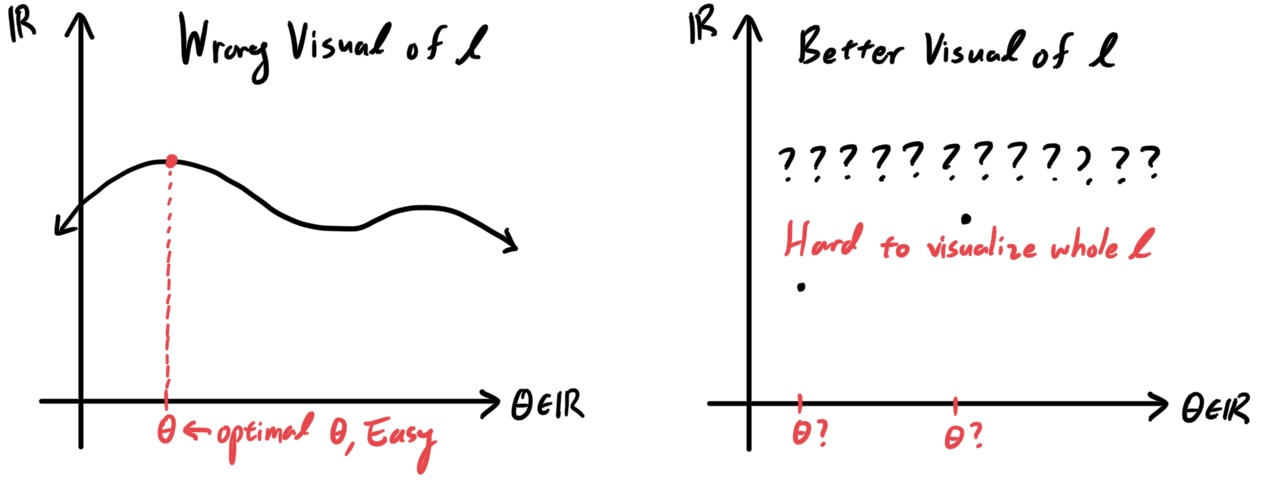
\includegraphics[width=0.6\textwidth]{img/visual_of_l.jpg}
    \caption{} 
    \label{fig:visual_of_l}
  \end{figure}

  Rather, all we can do is hope to take whatever easier-to-visualize, lower-bound functions and maximize them as much as we can in hopes of converging onto $l$. Let us walk through the first two iterations of the EM algorithm. We first initialize $\theta$ to, say $\theta_0$. This immediately induces the lower-bound ELBO-sum function $\sum_{i} \text{ELBO} (x^{(i)};\, p_Z^{*i}, \theta)$, which takes in multinomial density functions $p_Z^{*i} = p_1, p_2, \ldots$ and outputs different functions of $\theta$ that are valid lower bounds. Two of these possible lower-bound functions are shown (in green) for when we input some arbitrary density $p_1, p_2$. However, there exists a density $p_Z^{(i)}$ that produces not only the maximum possible lower-bound (called max ELBO, shown in red) but is equal to $l(\theta)$ for that density input $p_Z^{(i)}$. We maximize this function with respect to $\theta$ to get $\theta_1$ as our next assignment of $\theta$. 

  \begin{figure}[H]
    \centering 
    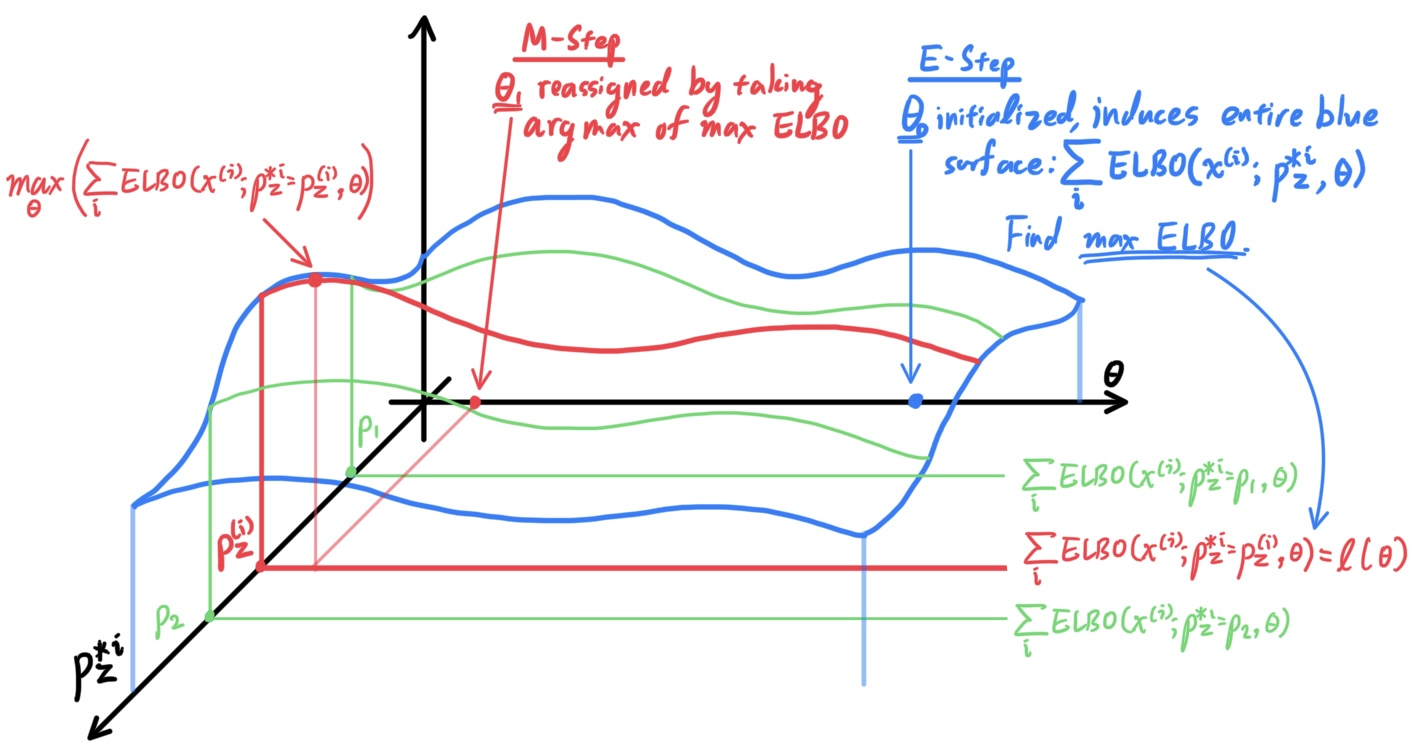
\includegraphics[width=0.7\textwidth]{img/EM_first_iteration.jpg}
    \caption{} 
    \label{fig:EM_first_iteration}
  \end{figure}

  The next step is identical. Now that we have a new value of $\theta = \theta_1$, this induces the lower-bound ELBO-sum function $\sum_{i} \text{ELBO} (x^{(i)};\, p_Z^{*i}, \theta)$ that also takes in multinomial densities $p_Z^{*i}$ and outputs different functions of $\theta$ that are valid lower-bounds. Two possible lower bounds are shown (in green), but the maximum lower-bound (in blue) is produced when we input density $p_Z^{(i)}$. Since this max ELBO function is equal to $\theta$ for this fixed density input $p_Z^{(i)}$, we maximize this function with respect to $\theta$ to get $\theta_2$ as our next assignment of $\theta$. 

  \begin{figure}[H]
    \centering 
    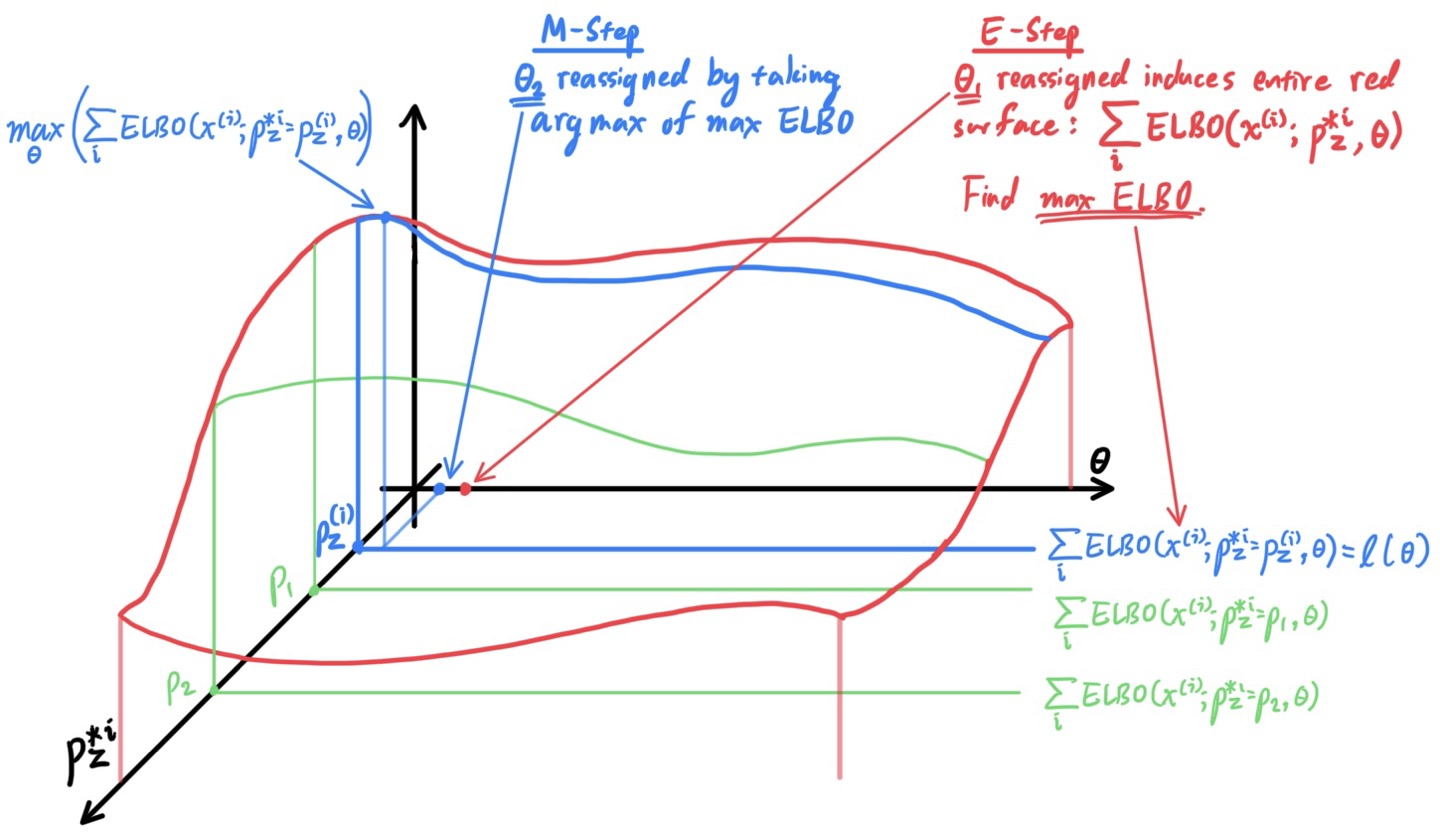
\includegraphics[width=0.7\textwidth]{img/EM_second_iteration.jpg}
    \caption{} 
    \label{fig:EM_second_iteration}
  \end{figure}

\subsection{Gaussian Mixture Models}

  Given a training set ${x^{(i)}}_{i=1}^n$ (without the $y$-labels and so in the unsupervised setting), there are some cases where it may seem like we can fit multiple Gaussian distributions in the input space $\mathcal{X}$. For example, the points below seem like they can be fitted well with 3 Gaussians.

  \begin{figure}[H]
    \centering
    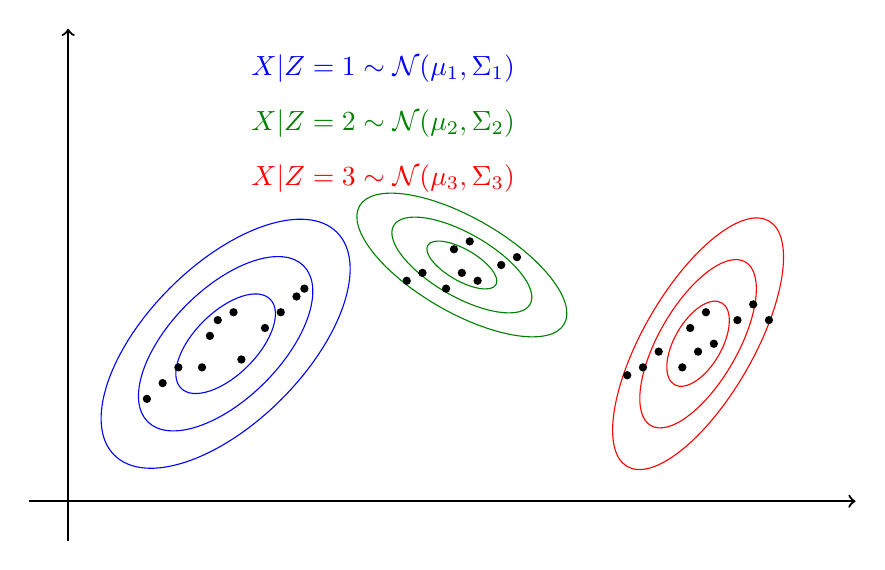
\begin{tikzpicture}
      % Draw axes
      \draw[black, ->, line width=0.8pt] (-0.5,0) -- (10,0);
      \draw[black, ->, line width=0.8pt] (0,-0.5) -- (0,6);
      
      % Equations at top
      \node[blue] at (4,5.5) {$X|Z=1 \sim \mathcal{N}(\mu_1, \Sigma_1)$};
      \node[green!50!black] at (4,4.8) {$X|Z=2 \sim \mathcal{N}(\mu_2, \Sigma_2)$};
      \node[red] at (4,4.1) {$X|Z=3 \sim \mathcal{N}(\mu_3, \Sigma_3)$};
      
      % First Gaussian (blue)
      \draw[blue, rotate around={45:(2,2)}] (2,2) ellipse (2 and 1);
      \draw[blue, rotate around={45:(2,2)}] (2,2) ellipse (1.4 and 0.7);
      \draw[blue, rotate around={45:(2,2)}] (2,2) ellipse (0.8 and 0.4);
      
      % Blue cluster points - more spread out
      \fill[black] (1.7,1.7) circle (1.5pt);
      \fill[black] (1.8,2.1) circle (1.5pt);
      \fill[black] (2.1,2.4) circle (1.5pt);
      \fill[black] (2.2,1.8) circle (1.5pt);
      \fill[black] (1.9,2.3) circle (1.5pt);
      \fill[black] (1.4,1.7) circle (1.5pt);
      \fill[black] (2.5,2.2) circle (1.5pt);
      \fill[black] (2.7,2.4) circle (1.5pt);
      \fill[black] (1.2,1.5) circle (1.5pt);
      \fill[black] (2.9,2.6) circle (1.5pt);
      \fill[black] (3.0,2.7) circle (1.5pt);
      \fill[black] (1.0,1.3) circle (1.5pt);
      
      % Second Gaussian (green)
      \draw[green!50!black, rotate around={-30:(5,3)}] (5,3) ellipse (1.5 and 0.6);
      \draw[green!50!black, rotate around={-30:(5,3)}] (5,3) ellipse (1 and 0.4);
      \draw[green!50!black, rotate around={-30:(5,3)}] (5,3) ellipse (0.5 and 0.2);
      
      % Green cluster points - more oval shaped
      \fill[black] (4.8,2.7) circle (1.5pt);
      \fill[black] (4.9,3.2) circle (1.5pt);
      \fill[black] (5.0,2.9) circle (1.5pt);
      \fill[black] (5.1,3.3) circle (1.5pt);
      \fill[black] (5.2,2.8) circle (1.5pt);
      \fill[black] (4.5,2.9) circle (1.5pt);
      \fill[black] (5.5,3.0) circle (1.5pt);
      \fill[black] (4.3,2.8) circle (1.5pt);
      \fill[black] (5.7,3.1) circle (1.5pt);
      
      % Third Gaussian (red)
      \draw[red, rotate around={60:(8,2)}] (8,2) ellipse (1.8 and 0.7);
      \draw[red, rotate around={60:(8,2)}] (8,2) ellipse (1.2 and 0.5);
      \draw[red, rotate around={60:(8,2)}] (8,2) ellipse (0.6 and 0.3);
      
      % Red cluster points - more spread out
      \fill[black] (7.8,1.7) circle (1.5pt);
      \fill[black] (7.9,2.2) circle (1.5pt);
      \fill[black] (8.0,1.9) circle (1.5pt);
      \fill[black] (8.1,2.4) circle (1.5pt);
      \fill[black] (8.2,2.0) circle (1.5pt);
      \fill[black] (7.5,1.9) circle (1.5pt);
      \fill[black] (8.5,2.3) circle (1.5pt);
      \fill[black] (7.3,1.7) circle (1.5pt);
      \fill[black] (8.7,2.5) circle (1.5pt);
      \fill[black] (8.9,2.3) circle (1.5pt);
      \fill[black] (7.1,1.6) circle (1.5pt);
    \end{tikzpicture}
    \caption{Example of data that can be fitted with 3 Gaussians}
  \end{figure}

  Therefore, we can construct a best-fit model as a composition of a multinomial distribution (to decide which one of the Gaussians $x$ should follow) followed by a Gaussian. 

  \begin{definition}[Gaussian Mixture Model] 
    The \textbf{Gaussian mixture model (GMM)} assumes that the covariates $x \sim X \in \mathbb{R}^d$ are generated by the following.\footnote{Therefore, our model says that each $x^{(i)}$ was generated by randomly choosing $z^{(i)}$ from ${1, \ldots, k}$ according to some multinomial, and then the $x^{(i)}$ was drawn from one of the $k$ Gaussians depending on $z^{(i)}$.} The parameters are $\theta = \{\lambda, \mu_1, \ldots, \mu_k, \Sigma_1, \ldots, \Sigma_k\}$.\footnote{Note that $\lambda$ really has $k-1$ free parameters and $\Sigma_i$'s should be symmetric and positive-definite.}

    \begin{enumerate}
      \item A latent variable $z \sim \mathrm{Multinomial}(\lambda)$, where $\lambda = (\lambda_1, \ldots, \lambda_k)$ with PMF defined 
      \begin{equation}
        p_\theta (z) = \lambda_z
      \end{equation}

      \item The generative random variable $X \mid Z = z \sim \mathcal{N}(\mu_i, \Sigma_i)$ where $\mu_z \in \mathbb{R}^d, \Sigma_z \in \mathbb{R}^{d \times d}$ and PDF defined 
      \begin{equation}
        p_\theta (x \mid z) = \frac{1}{(2\pi)^{d/2}|\Sigma_z|^{1/2}} \exp\left(-\frac{1}{2}(x-\mu_z)^\top\Sigma_z^{-1}(x-\mu_z)\right)
      \end{equation}
    \end{enumerate}
  \end{definition}

  We can write down the log-likelihood of the given data $x^{(i)}$'s as a function of all the parameters above as
  \begin{equation}
    \sum_{i=1}^n \log p_\theta (x^{(i)}) = \sum_{i=1}^n \log \bigg( \sum_{z=1}^k  p_\theta ( x^{(i)} \mid z^{(i)} ) , p_\theta ( z^{(i)} ) \bigg)
  \end{equation}

  \begin{example}[Dual Nature of Latents and Parameters]
    Note that since we only know that the \textit{final} value of the $i$th sample is $x^{(i)}$ and not anything at all about which value $z^{(i)}$ the $i$th sample had, there is an extra unknown in this model. If we did know the values of the hidden variables $z^{(i)}$ (i.e. if we knew which of the $k$ Gaussians each $x^{(i)}$ was generated from), then our log likelihood function would be much more simple since now, our givens will be both $x^{(i)}$ \textit{and} $z^{(i)}$. Therefore, we don't have to condition on the $z^{(i)}$ and can directly calculate the log of the probability of us having sample values $(z^{(1)}, x^{(1)}), (z^{(2)}, x^{(2)}), \ldots, (z^{(n)}, x^{(n)})$.

    \begin{equation}
      \sum_{i=1}^n \log p(x^{(i)}) = \sum_{i=1}^n \log p( x^{(i)}, z^{(i)}) = \sum_{i=1}^n \log p( x^{(i)} \mid z^{(i)}) \, p(z^{(i)})
    \end{equation}

    This model, with known $z^{(i)}$'s, is basically the GDA model, which is easy to calculate. That is, the maximum values of $\phi, \mu, \Sigma$ are

    \begin{align*}
      \phi_j & = \frac{1}{n} \sum_{i=1}^n \mathbbm{1}_{z^{(i)} = j} \\
      \mu_j & = \frac{\sum_{i=1}^n \mathbbm{1}_{z^{(i)} = j} x^{(i)}}{\sum_{i=1}^n \mathbbm{1}_{z^{(i)} = j}} \\
      \Sigma_j & = \frac{1}{\sum_{i=1}^n \mathbbm{1}_{z^{(i)} = j}} \sum_{i=1}^n \mathbbm{1}_{z^{(i)}} \big( x^{(i)} - \mu_j \big),\big(x^{(i)} - \mu_j \big)^T
    \end{align*}
  \end{example}

  But since we do \textit{not} know the values of $z^{(i)}$, we first try to ``guess'' the values of the $z^{(i)}$'s and then update the parameters of our model assuming our guesses are correct. 

  \begin{algo}[EM Algorithm on GMMs]
    The EM Algorithm applied to GMMs has the following steps:

    \begin{enumerate}
      \item Randomly initialize $\theta^{[0]} = \{\lambda, \mu_1, \ldots, \mu_k, \Sigma_1, \ldots, \Sigma_k\}$.\footnote{This might converge faster using K-means initialization.} 

      \item \textbf{(E Step)} Calculate the posterior density $p(z \mid x)$ by applying Bayes rule to each sample keeping the parameter $\theta^{[t]}$ fixed. 
      \begin{equation}
        p_{\theta^{[t]}} (z \mid x^{(i)}) = \frac{p_{\theta^{[t]}} (x^{(i)} \mid z) \, p_{\theta^{[t]}}(z)}{p(x)} = \frac{p_{\theta^{[t]}} (x^{(i)} \mid z) \, p_{\theta^{[t]}}(z)}{\sum_z p_{\theta^{[t]}} (x^{(i)} \mid z) \, p_{\theta^{[t]}}(z)}
      \end{equation}
      We should have $n$ different multinomial distribution parameters, each representing our best guess of what multinomial density $p(z \mid x^{(i)})$ each $x^{(i)}$ had followed in order to be at the given points. Let's label the updated parameters of the multinomial distribution of the $i$th sample to be $\lambda^{[t](i)}$ at the $t$th iteration. 

      \item \textbf{(M Step)} We update $\theta$ as such. 
      \begin{align}
        \lambda^{[t+1]}  & = \frac{1}{n} \sum_{i=1}^n \lambda^{[t](i]} \\
        \mu_j^{[t+1]} & = \frac{\sum_{i=1}^n \lambda^{[t](i]}_j x^{(i)}}{\sum_{i=1}^n \lambda^{[t](i)}} \\ 
        \Sigma_j^{[t+1]} & = \frac{1}{\sum_{i=1}^n \lambda^{[t](i]}} \sum_{i=1}^n \lambda^{[t](i)}_j \,\big(x^{(i)} - \mu_j^{[t+1]} \big]\big(x^{(i)} - \mu_j^{[t+1]} \big]^T
      \end{align}

      \item Repeat steps 2 and 3 until convergence. 
    \end{enumerate}
  \end{algo}

  Let us elaborate further on the intuition of this step. In the normal GDA with given values of $z^{(i)}$, we have $\lambda= \frac{1}{n} \sum_{i=1}^n 1\{z^{(i)} = j\} = \frac{1}{n}\big(\text{Number of Samples in }j\text{th Gaussian}\big)$, which is a sum of "hard" guesses, meaning that each $x^{(i)}$ is undoubtedly in cluster $j$ or not, and so to find out our best guess for the true vector $\lambda$, all we have to do is find out the proportion of all examples in each of the $k$ groups and we're done (without needing to iterate). However, in our EM model, we do not know the $z^{(i)}$'s, and so the best we can do is give the \textit{probability} $\lambda^{(i)}_j$ that $x^{(i)}$ is in cluster $j$. So for each point $x^{(i)}$, the model has changed from it being undoubtedly in group $z^{(i)} = j$ to it having a probability of being in $\lambda^{(i)}_j$ for $j = 1, \ldots, k$.

  \begin{figure}[H]
    \centering
    \begin{subfigure}[b]{0.48\textwidth}
      \centering
      \begin{tikzpicture}[scale=1.]
        \draw[->] (-0.5,0) -- (5,0);
        \draw[->] (0,-0.5) -- (0,3.5);
        
        % Points and labels
        \fill[red] (1,1) circle (3pt);
        \fill[red] (1.5,0.8) circle (3pt);
        \fill[red] (2,1.5) circle (3pt);
        \node[red] at (3,1.5) {$\lambda=\frac{3}{6}$};
        
        \fill[blue] (3,2.5) circle (3pt);
        \fill[blue] (3.2,2) circle (3pt);
        \node[blue] at (4,2.5) {$\lambda=\frac{2}{6}$};
        
        \fill[green!50!black] (4,1) circle (3pt);
        \node[green!50!black] at (4.5,1) {$\lambda=\frac{1}{6}$};
      \end{tikzpicture}
      \caption{Hard label assignments.}
      \label{fig:hard-guesses}
    \end{subfigure}
    \hfill 
    \begin{subfigure}[b]{0.48\textwidth}
      \centering
      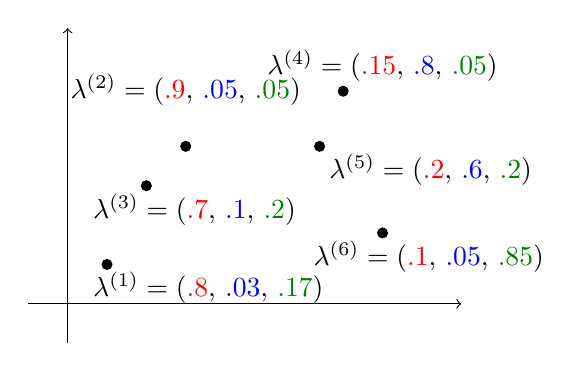
\begin{tikzpicture}[scale=1]
        \draw[->] (-0.5,0) -- (5,0);
        \draw[->] (0,-0.5) -- (0,3.5);
        
        % Points and colored vectors
        \fill (0.5,0.5) circle (2pt);
        \node[right] at (0.2,0.2) {$\lambda^{(1)} = ($\textcolor{red}{.8}, \textcolor{blue}{.03}, \textcolor{green!50!black}{.17}$)$};
        
        \fill (1.5,2) circle (2pt);
        \node[above] at (1.5,2.4) {$\lambda^{(2)} = ($\textcolor{red}{.9}, \textcolor{blue}{.05}, \textcolor{green!50!black}{.05}$)$};
        
        \fill (1,1.5) circle (2pt);
        \node[right] at (0.2,1.2) {$\lambda^{(3)} = ($\textcolor{red}{.7}, \textcolor{blue}{.1}, \textcolor{green!50!black}{.2}$)$};
        
        \fill (3.5,2.7) circle (2pt);
        \node[above] at (4,2.7) {$\lambda^{(4)} = ($\textcolor{red}{.15}, \textcolor{blue}{.8}, \textcolor{green!50!black}{.05}$)$};
        
        \fill (3.2,2) circle (2pt);
        \node[right] at (3.2,1.7) {$\lambda^{(5)} = ($\textcolor{red}{.2}, \textcolor{blue}{.6}, \textcolor{green!50!black}{.2}$)$};
        
        \fill (4,0.9) circle (2pt);
        \node[right] at (3,0.6) {$\lambda^{(6)} = ($\textcolor{red}{.1}, \textcolor{blue}{.05}, \textcolor{green!50!black}{.85}$)$};
      \end{tikzpicture}
      \caption{Soft probability assignments.}
      \label{fig:soft-guesses}
    \end{subfigure}
    \caption{The superscript $[t]$ is omitted for clarity.}
    \label{fig:guesses-comparison}
  \end{figure}

  When we update the $\lambda$ in the M-step, we can interpret the vectors $\lambda^{(i)}$ as tuples where $\lambda^{(i)}_j$ describes the expected "portion" of each sample $x^{(i)}$ to be in group $j$. So, we are adding up all the "portions" of the points that are expected to be in cluster $j$ to get $\lambda= \sum_{i=1}^n \lambda^{(i)}$. 

  \begin{figure}[H]
    \centering 
    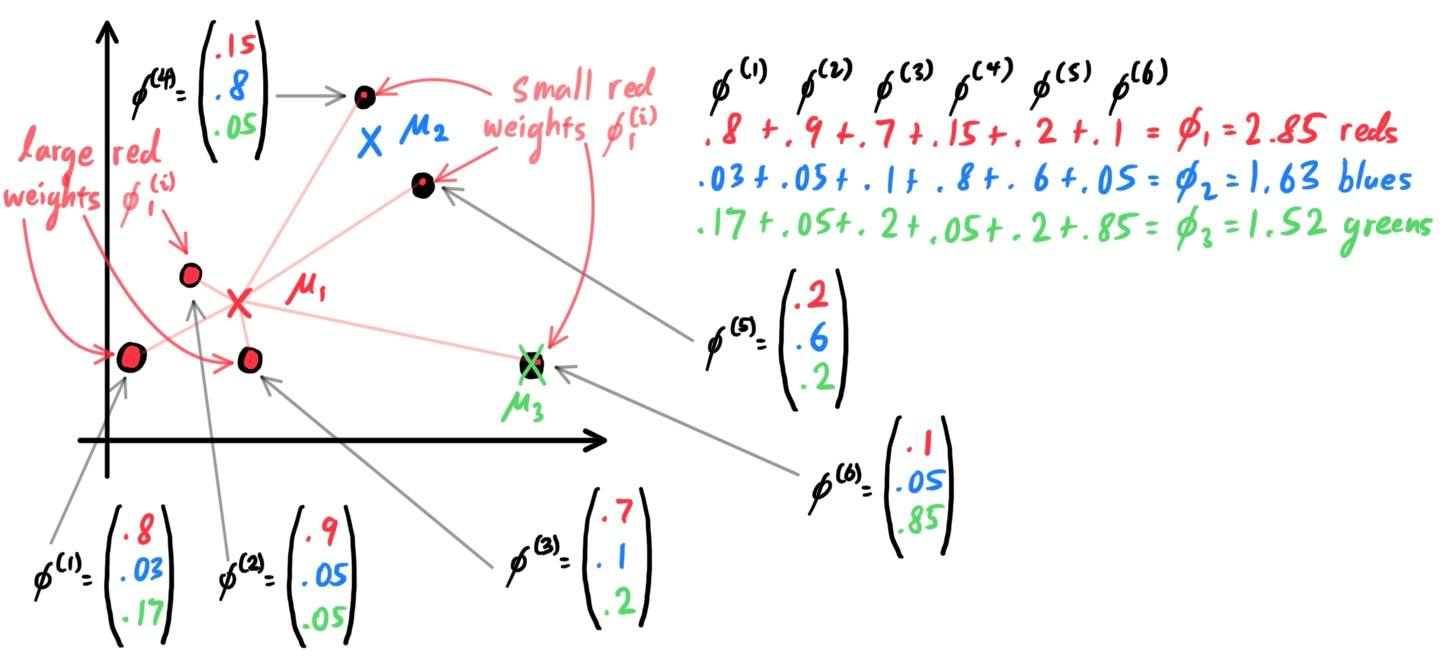
\includegraphics[scale=0.2]{img/weighted_means.jpg}
    \caption{}
    \label{fig:weighted_means}
  \end{figure}

  Now, given the $j$th Gaussian cluster, we would like to compute its mean $\mu_j$. Since each $x^{(i)}$ has probability $\lambda^{(i)}_j$ of being in cluster $j$, we can weigh each of the $n$ points by $\lambda^{(i)}_j$ (which determines how "relevant" $x^{(i)}$ is to cluster $j$) and average these (already weighted) points to get our "best-guess" of the mean $\mu_j$. Given the MLE of the means, we can straightforwardly compute the MLE of the covariance matrices. 

  In summary, this entire algorithm results from modifying the ``hard'' data of each point $x^{(i)}$ being undoubtedly in one cluster to a model containing points $x^{(i)}$ that have been "smeared" around different clusters, with a probability $\lambda^{(i)}$ being in cluster $j$. 

\subsection{Nonlinear ICA} 
